\documentclass[runningheads]{llncs}
\usepackage[utf8]{inputenc}
\usepackage{amsmath}
\usepackage{amsfonts}
\usepackage{subfiles}
\usepackage{amssymb}
\usepackage{csquotes}
\usepackage[numbers, sort, comma, square]{natbib}
\usepackage{changepage}
\usepackage{graphicx}
\usepackage{placeins}
\usepackage{xr}
\usepackage{tabularx}
\usepackage{lscape}
\usepackage{hyperref}
\usepackage{tablefootnote}
\usepackage{fancyhdr}
\usepackage{hyperref}
\newenvironment{jumpin}{\begin{adjustwidth}{0.3in}{}}{\end{adjustwidth}}
\newcolumntype{R}[1]{>{\raggedleft\let\newline\\\arraybackslash\hspace{0pt}}m{#1}}


\begin{document}
\title{Document Embedding for Scientific Articles:\newline A validation of word embeddings}
\titlerunning{Document embedding for Scientific Articles}

\author{H.J. Meijer\inst{1,2}\orcidID{0000-1111-2222-3333} \and
R. Karimi\inst{2}\orcidID{1111-2222-3333-4444}}
\authorrunning{H.J. Meijer et al.}

\institute{University of Amsterdam, Science park 904, 1012WX Amsterdam, The Netherlands \and
Elsevier, Radarweg 29, 1043 NX Amsterdam, The Neterlands
\email{meijerarjan@live.nl, r.karimi@elsevier.com}}
\maketitle

\begin{abstract}
Over the last few years, word embeddings have taken a dominant position in the information retrieval research. Studies conducted have focused on the quality and application of word embeddings on corpuses such as Wikipedia or online comments/reviews/tweets. However, these studies are limited to generic texts and lack technical, scientific or domain specific nuances such as rare words, lots of abbreviations, or chemical/mathematical formulas commonly used in academic context. This research focusses on the quality and application of word embeddings on academic corpuses. Word embedding requires less memory and is processed faster than conventional alternatives such as TFIDF. Hence, we intend to use word embeddings as an efficient way to model the content for our recommendation/disambiguation/search engines. This study focuses on word embedding compared to TFIDF for modeling content in scientific articles. We use a word2vec model  trained on titles and abstracts of roughly 68 millions scientific articles. Word embedding are evaluated against existing benchmarks for generic texts from previous studies. Furthermore, we have developed a new benchmark to evaluate these embedding in the scientific context. We validate the word embeddings via a categorization task to match articles to journals for roughly 1.4 millions articles published in 2017. Our results show that word embedding is a better content model for titles (short text) while TFIDF is a better model for abstracts (longer text).
\keywords{Word Embedding  \and Document Embedding \and Article Embedding \and Journal Embedding \and Embedding Visualization \and Embedding Validation.}
\end{abstract}
\section{Introduction}
Over the last few years word embeddings have proven to be powerful tools. Word embeddings, numerical representations of words, have atraccted the attention of many researchers over the last few years. Embeddings, created by (unsupervised) machine learning models\cite{lai2016generate} are able to capture semantic and syntactic information about words\cite{mikolov2013distributed}. The usage of word embeddings has improved various Natural Language Processing areas such as named entity recognition, part-of-speech tagging, parsing, and semantic role labelling~\cite{luong2013better}. Embeddings can furthermore be used in search and recommendation. Potential application of the embeddings in the academic domain could be the improvement of search engines, text analysis to improve NLP tasks for academic texts, and journal recommendation for publishing articles. Studies till this day have mostly focussed on generic texts like Wikipedia, or informal texts like reviews and tweets. We aim to validate the word embeddings for academic texts, containing technical, scientific or domain specific nuances such as rare words, lots of abbreviations, or chemical/mathematical formulas. We validate the embeddings by matching articles to journals, ranking them on cosine-similarity.
\section{Data \& Environment}
For this research we used a dataset consisting of $186.962.354$ tokens. These tokens have been collected from $1.391.543$ articles which have been published in $3.759$ distinct journals. In our dataset, each article is represented with a title and an abstract. The word occurrences in our dataset follow a Pareto-like distribution as described by \citet{wiegand2018word}, indicating that our original data has the same properties as standard English texts. We used Spark for this research, enabeling us to use its tools for big data processing\cite{armbrust2015spark}.
\subsection{Sets}
\subsubsection{Embeddings}
We used 300-dimensional embeddings, created by \citet{Truong2017Thesis}, based on the Word2Vec model. From these embeddings we created multiple embedding sets. These sets are: the default embedding; as created by \citet{Truong2017Thesis} and TF-IDF weighted embeddings (referred to in figures as \textit{embedding}). We used 4 variants of TF-IDF weighted embeddings: 
\begin{itemize}
\item{TF-IDF embedding (\textit{TFIDF\_embedding}); all words, weighted with the TF-IDF score, averaged to create an article embedding.}
\item{10K embedding (\textit{10K\_embedding}); TF-IDF weighting limited to the top 10.000 most occurring tokens.}
\item{5K embedding (\textit{5K\_embedding}); TF-IDF weighting limited to the top 5.000 most occurring tokens.}
\item{1K 6K embedding (\textit{1K\_6LK\_embedding}); TF-IDF weighting limited to the top 1.000 till 6.000 most occurring tokens.}
\end{itemize}
\subsubsection{TFIDF}
We furthermore used 3 TF-IDF sets, to create these sets we used the TF-IDF model and a hasher from the PySpark MlLib\footnote{\url{http://spark.apache.org/docs/2.0.0/api/python/pyspark.mllib.html}.}. We controlled these sets in two ways, (a) adjusting vocabulary size of the input and (b) adjusting the number of hashbuckets. We label the TF-IDF sets as follows: "vocabulary size / number of hash buckets", we furthermore indicate 1.000 as 1K. Thus, we label the TF-IDF configuration that has a vocabulary size of 10.000 and 10.000 hash buckets as TF-IDF 10K/10K. To select the TF-IDF sets, we measured and memory usage of multiple TF-IDF configurations. These results can be seen in Figures~\ref{figure:tfidfPerformance} and~\ref{figure:tfidfMemory}, in this figure we can see that the performance on both title and abstract stagnates; the same is true for the memory usage, although the memory usage does not stagnate as fast as the performance. Given these results, we selected the 10K/10K, 10K/5K and 5K/5K configurations for our research.
\begin{figure}[hbt]
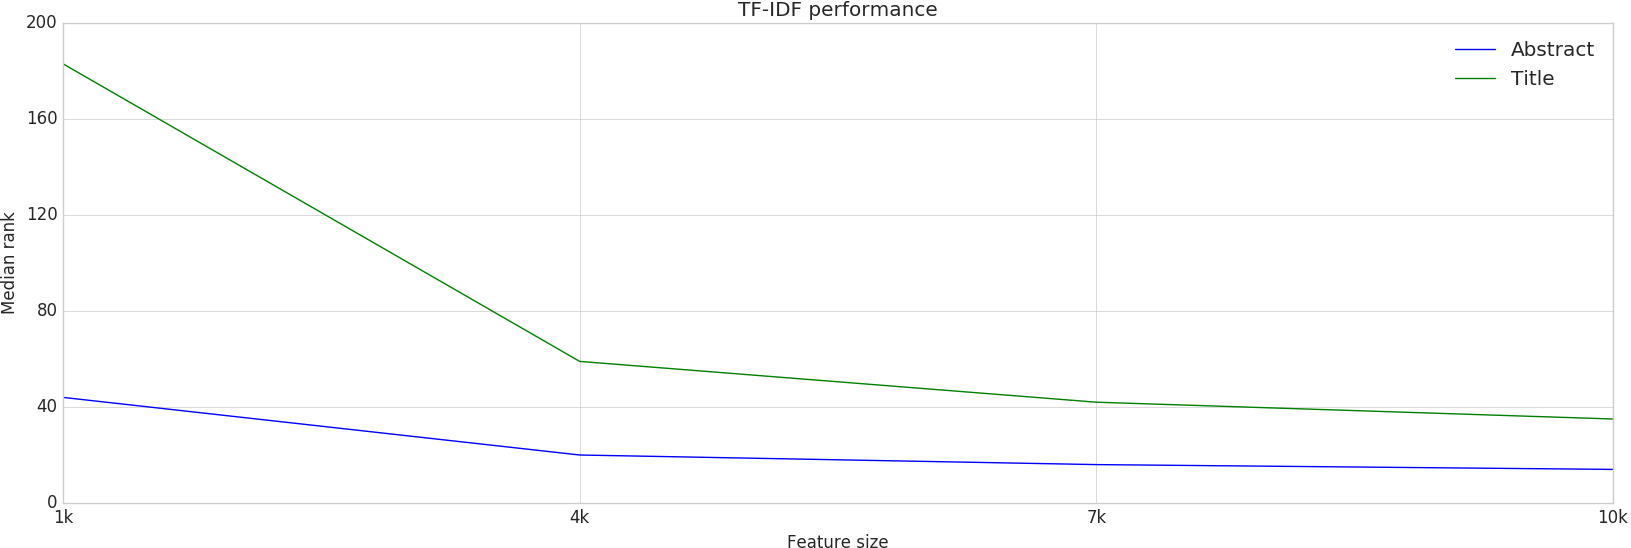
\includegraphics[width=5in]{Plots/tfidf_selection_plot_performance}
\caption{TF-IDF performance on title and abstract.}\label{figure:tfidfPerformance}
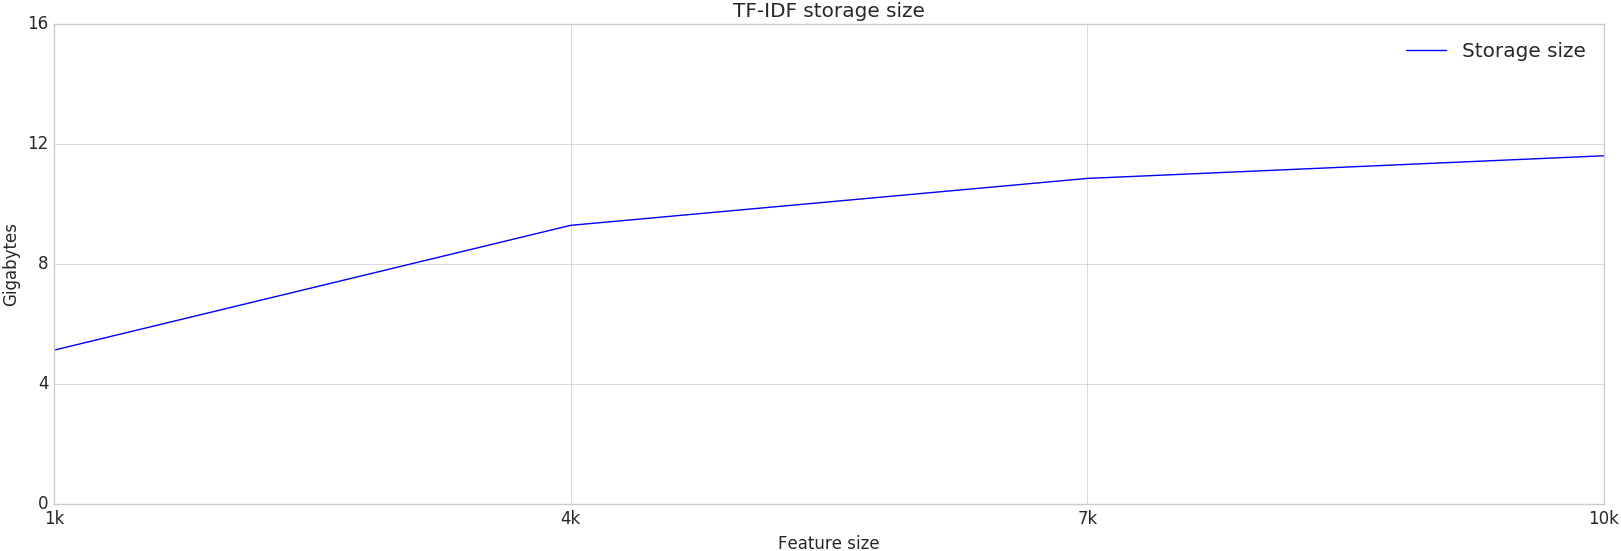
\includegraphics[width=5in]{Plots/tfidf_selection_plot_memory}
\caption{TF-IDF memory usage for title and abstract combined.}\footnote{We combined the memory usage of the titles and abstracts since the titles and abstract are created together and share their feature vector size.}\label{figure:tfidfMemory}
\end{figure}
\FloatBarrier
\section{Methodology}
We use a ranking task to validate the quality of the different sets. We calculate the distance from each article from our validation set to each journal embedding from our training set. We then order the journals (ascending) based on their similarity. We use as ranking the rank of the journal from which the article was taken (source journal) in the resulting list. We do this for both title and abstract separately.\\
We calculate the performance per set, therefore we combine the ranking results of all articles for a set into one score. We use the median and average for that; where the average rank takes the total average of all ranks, the median is the point at which 50\% of all the ranks are greater and 50\% of all the ranks are lower than the point. We keep track of the following results when ranking: source journal rank and best match journal for both abstract and title. We furthermore monitor the memory usage and computation time.
\section{Results}
In this section the results of our research are presented; the detailed discussion on the meaning and implications of these results are presented in XXXXXXXXX discussion.
\subsection{Ranking}
The Figures~\ref{figure:titleRanks} \&~\ref{figure:abstractRanks} show the result of the categorization task as ranking results. The rank indicates the position of the correct journal in the sorted list of matched journals. Figure~\ref{figure:titleRanks} shows the ranking results for the different sets based on the title. Figure~\ref{figure:abstractRanks} displays the ranking results based on the abstract. Both graphs show both average and median ranks, based on the cosine-similarity between the article and journal embeddings or feature vectors.
\subsection{Rank distribution}
Figures~\ref{figure:titleDistribution} and~\ref{figure:abstractDistribution} show the distributions of the ranks for each set. The Figures plot the summed amount of articles against the ranks on a logarithmic scale. Figure~\ref{figure:titleDistribution} shows the rank distribution for the titles, Figure~\ref{figure:abstractDistribution} shows this for the ranks based on the abstract. These graphs give a detailed view of the ranks presented in their respective figures (Figures~\ref{figure:titleRanks} and~\ref{figure:abstractRanks}).
\subsection{F1-Score}
Figures~\ref{figure:f1Title} and~\ref{figure:f1Abstract} show the precision, recall and F1 scores. These scores are calculated on journal level, and are averaged per set. Figure~\ref{figure:f1Title} shows the F1 score for the title and Figure~\ref{figure:f1Abstract} shows the scores for the abstract. These scores indicate the performance of the sets on absolute hits/top-1.
\subsection{Memory usage}
Table~\ref{table:memoryUsage} shows the total memory usage of each set for the \textit{Validation set}, indicating their storage costs in gigabytes\footnote{1024 based}. It furthermore shows the absolute hit percentage of the title and the abstracts, i.e. the percentage of articles that have their source\footnote{Journal from which the article was taken} journal as the first result in the ranking. The table furthermore shows the median rank and the median abstract rank, as visualized in Figures \ref{figure:titleRanks} and~\ref{figure:abstractRanks}. Thus, this table gives an overview of the memory usage of the sets, combined with their performance on the ranking task.
\subsection{Computation Time}
Table~\ref{table:computationTimes} shows the computation time needed for 1.000 distance calculations, based on the cosine-similarity distance measurement. 1.000 vectors (V) have been randomly selected and transformed into a matrix (M). We then calculate the distance between each vector from V to the matrix M; this results in the distance between the vector an all vectors (V) contained in the matrix (M). We do this for all vectors in V, for the 10K/10K TF-IDF set and the default embeddings. Because the embeddings are dense vectors, we also transformed the TF-IDF feature vectors to dense vectors for this comparison. Table~\ref{table:computationTimes} shows both computation time in seconds and the embedding fraction; meaning how many times faster the embedding is, based on time in seconds.
\FloatBarrier
\begin{figure}
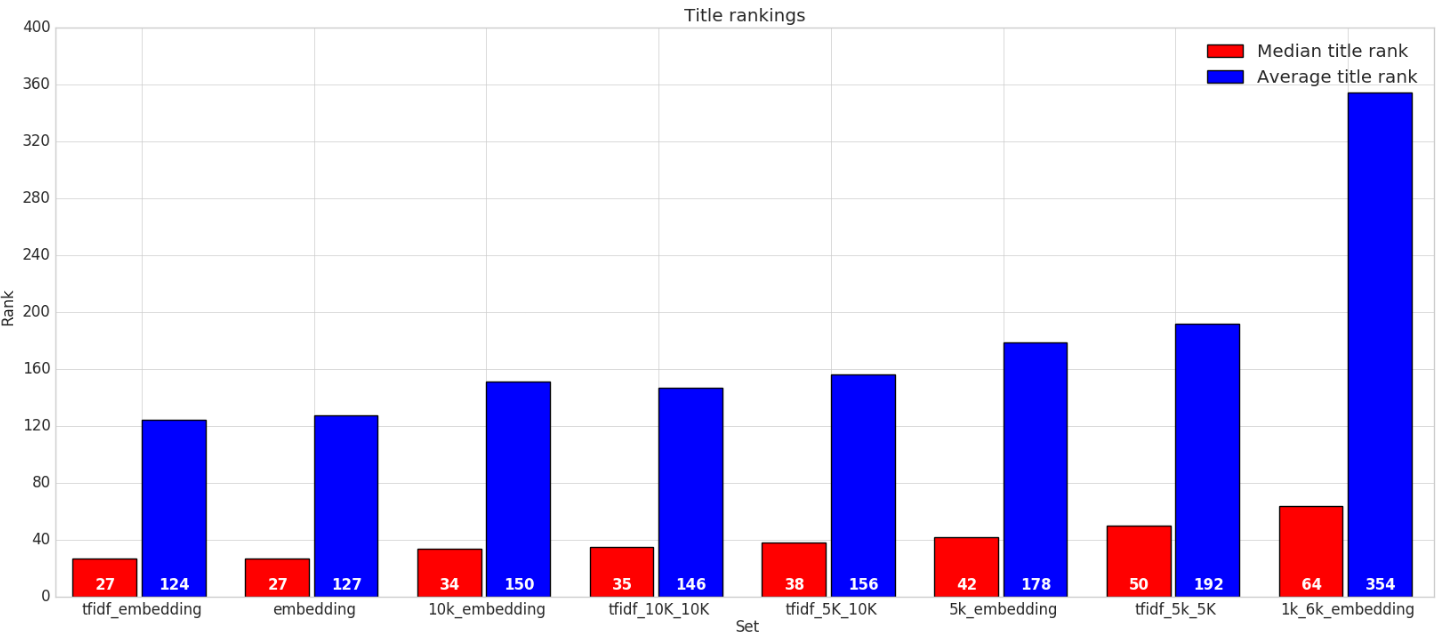
\includegraphics[width=4.5in]{Plots/Title_rankings}
\caption{Median and average title rankings}\label{figure:titleRanks}
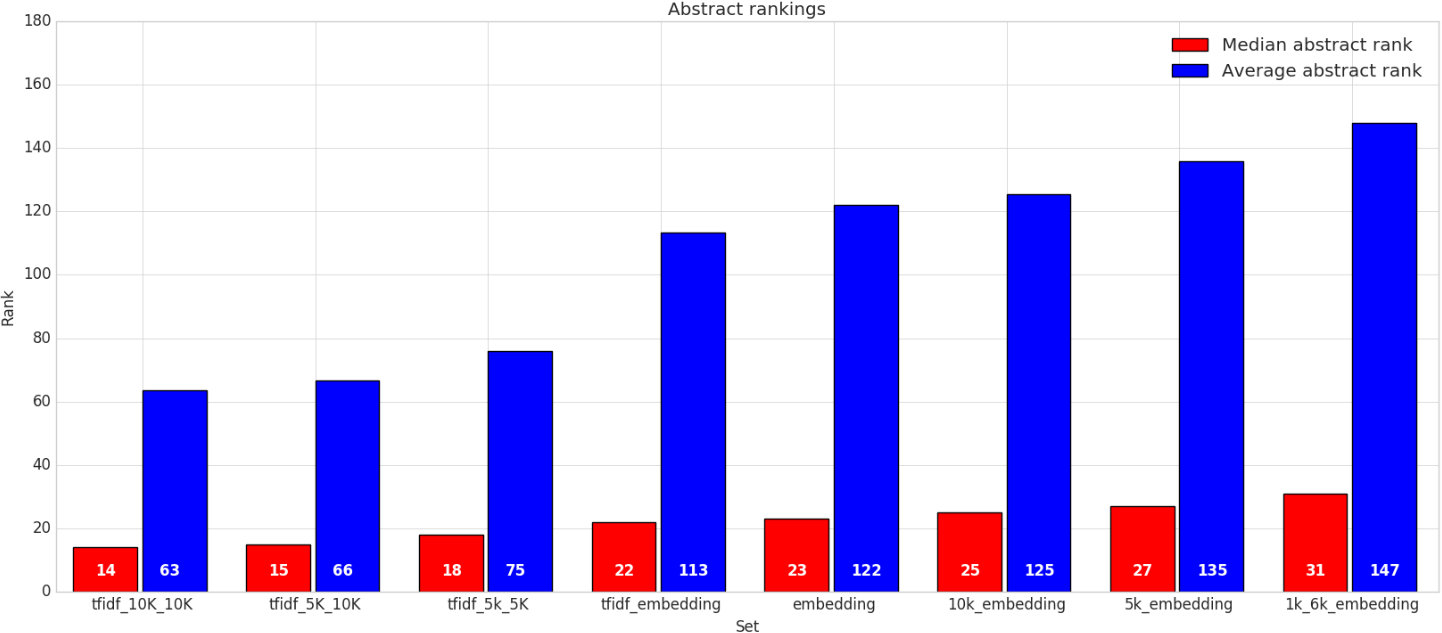
\includegraphics[width=4.5in]{Plots/Abstract_rankings}
\caption{Median and average abstract rankings}\label{figure:abstractRanks}
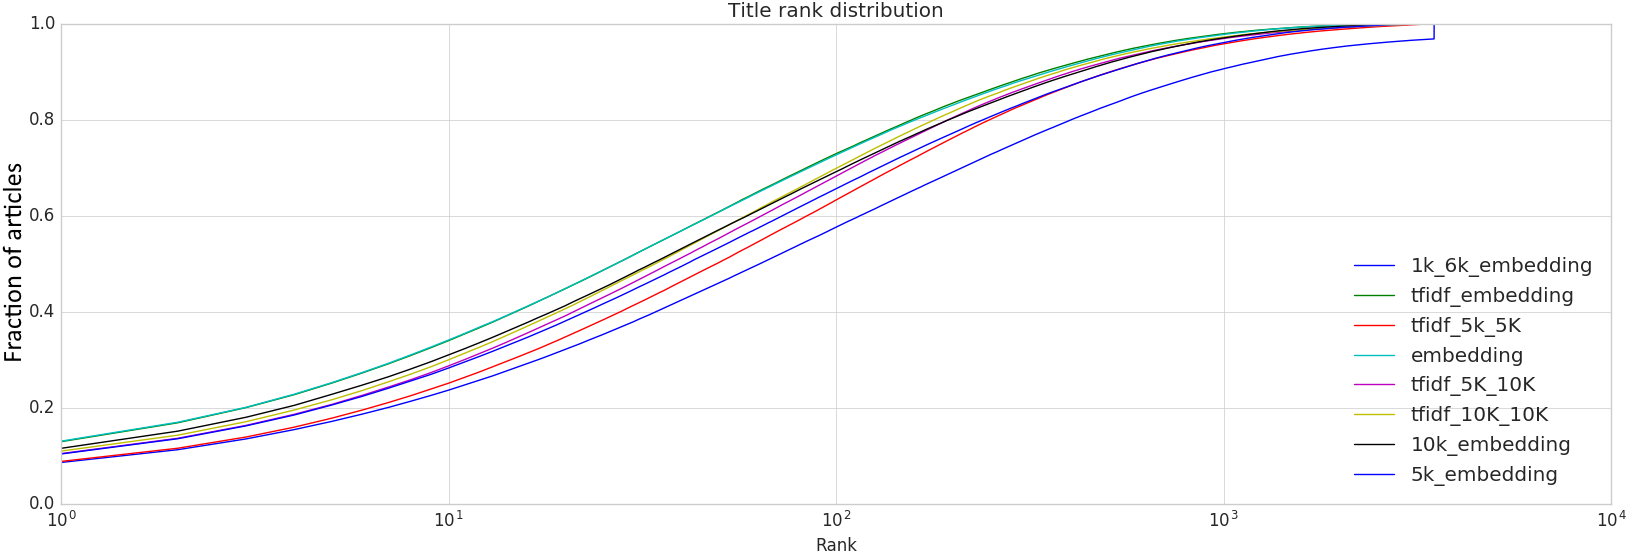
\includegraphics[width=4.5in]{Plots/Title_rank_distribution}
\caption{Title rank distribution per set, Y-axis shows the fraction of articles.}\label{figure:titleDistribution}
\end{figure}
\begin{figure}
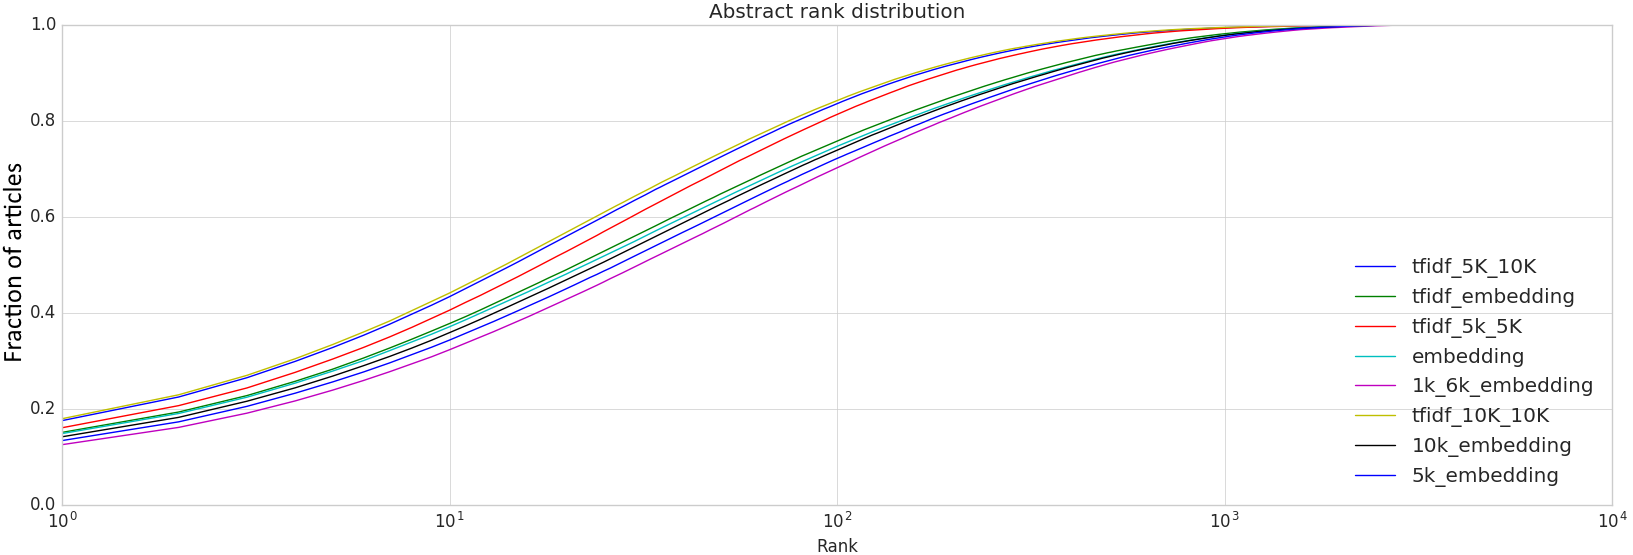
\includegraphics[width=4.5in]{Plots/Abstract_rank_distribution}
\caption{Abstract rank distribution per set, Y-axis shows the fraction of acticles.}\label{figure:abstractDistribution}
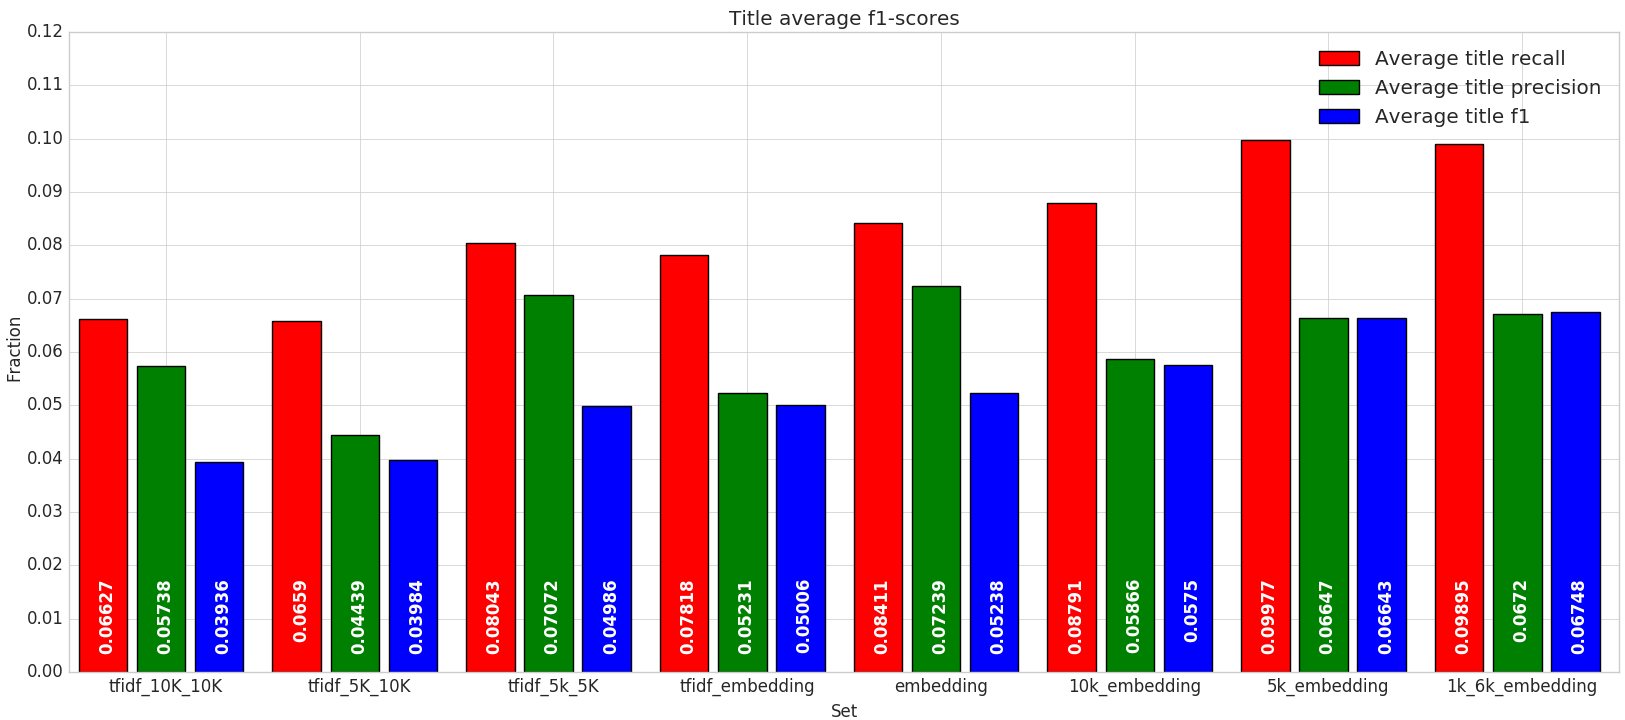
\includegraphics[width=4.5in]{Plots/Title_avg_f1}
\caption{Precision, recall and F1 scores based on title}\label{figure:f1Title}
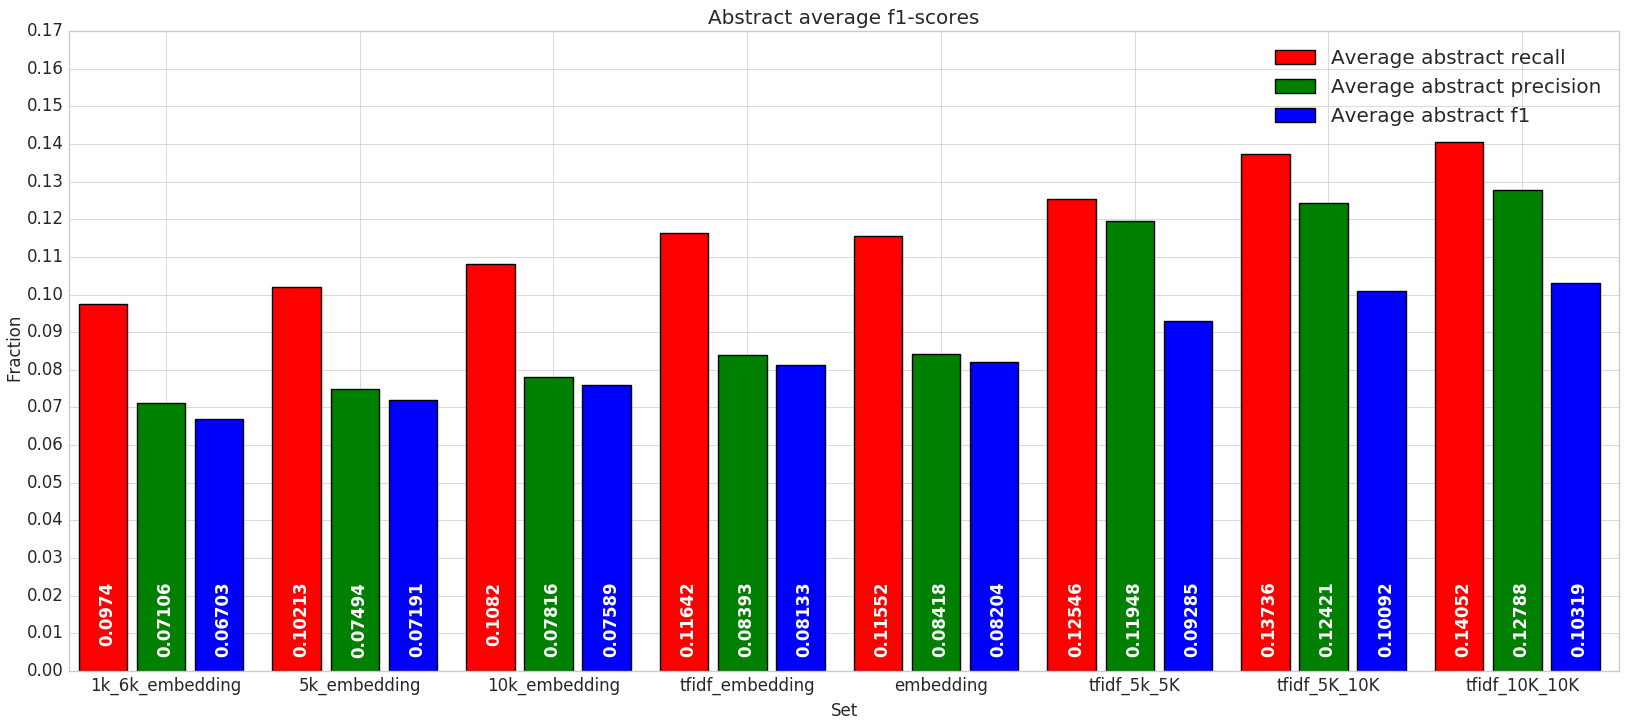
\includegraphics[width=4.5in]{Plots/Abstract_avg_f1}
\caption{Precision, recall and F1 scores based on abstract}\label{figure:f1Abstract}
\end{figure}
\FloatBarrier
\begin{center}
\begin{table}
\begin{tabular}{|l|r|r|r|r|}
\hline
Set & Size in GB & Absolute hit percentage & Median title rank & Median abstract rank\\
&&\begin{tabular}{p{0.5in}|p{0.5in}}Title & Abstract\end{tabular}&&\\
\hline
tfidf 5k 5K & $9.82$ & \begin{tabular}{R{0.5in}|R{0.5in}}5.42\% & 10.18\%\end{tabular} & 50 & 27\\
\hline
tfidf 5K 10K & $11.47$ & \begin{tabular}{R{0.5in}|R{0.5in}}6.49\% & 11.08\%\end{tabular} & 38 & 15\\
\hline
\textbf{tfidf 10K 10K} &\textbf{11.61}& \begin{tabular}{R{0.5in}|R{0.5in}}\textbf{6.79\%} & \textbf{11.32\%}\end{tabular} & \textbf{35} & \textbf{14}\\
\hline
embedding & $3.13$ & \begin{tabular}{R{0.5in}|R{0.5in}}7.92\% & 9.24\%\end{tabular} & 27 & 23\\
\hline
5k embedding & $3.13$ & \begin{tabular}{R{0.5in}|R{0.5in}}6.34\% & 8.36\%\end{tabular} & 42 & 27\\
\hline
10k embedding & $3.13$ & \begin{tabular}{R{0.5in}|R{0.5in}}7.03\% & 8.76\%\end{tabular} & 34 & 25\\
\hline
\textbf{tfidf embedding} & \textbf{3.13} & \begin{tabular}{R{0.5in}|R{0.5in}}\textbf{7.89\%} & \textbf{9.33\%}\end{tabular} & \textbf{27} & \textbf{22}\\
\hline
1k 6k embedding & $3.06$ & \begin{tabular}{R{0.5in}|R{0.5in}}5.16\% & 7.86\%\end{tabular} & 64 &31 \\
\hline
\end{tabular}
\caption{Memory usage and performance for each set}\label{table:memoryUsage}
%\end{table}
%\begin{table}
\begin{tabular}{|p{1.5in}|p{1.65in}|p{1.2in}|}
\hline
 & Computation time (seconds) & Embedding fraction\\
 & \begin{tabular}{R{0.77in}|R{0.82in}}Title & Abstract\end{tabular} & \begin{tabular}{R{0.5in}|R{0.6in}}Title & Abstract\end{tabular} \\
\hline
TF-IDF (sparse vector) & \begin{tabular}{R{0.77in}|R{0.82in}} 154.95 & 169.89 \end{tabular}& \begin{tabular}{R{0.5in}|R{0.6in}} 231.25 & 184.36\end{tabular}\\
\hline
TF-IDF (dense vector) &\begin{tabular}{R{0.77in}|R{0.82in}} 35.67 & 35.18 \end{tabular} & \begin{tabular}{R{0.5in}|R{0.6in}} 53.23 & 39.59 \end{tabular} \\
\hline
Embedding & \begin{tabular}{R{0.77in}|R{0.82in}} 0.67&0.89 \end{tabular}& \begin{tabular}{R{0.5in}|R{0.6in}}1&1\end{tabular}\\
\hline
\end{tabular}
\caption{Comparison of computation time in seconds, based on 1.000 distance calculations. Showing both absolute measurements and the fraction to the embedding time.} \label{table:computationTimes}
\end{table}
\end{center}
\FloatBarrier
\section{Discussion}
\subsection{Results analysis}
\subsubsection{Best performers}
The data, as presented in Figures~\ref{figure:titleRanks} and~\ref{figure:abstractRanks} shows that the 10k/10k set performs better than all other TF-IDF sets, although the difference with the 5k/10k is low, 1  median rank on abstract and 3 median ranks on the titles. For the embeddings, the TF-IDF weighted embedding works better than the others, although it is not a significant improvement (1 rank on a set of more than 3.000) compared to the default embeddings, which is 1 median rank higher on the abstracts, and equal on the titles. 
\subsubsection{TF-IDF}
The TF-IDF feature vectors outperform the embeddings on the abstracts, while the embeddings outperform the TF-IDF feature vectors on the titles. The main difference between the abstract and title is that the title contains fewer tokens compared to the abstract (see Table~\ref{table:corpusSize}). This means that the titles contain less information than the abstracts. Due to this, the TF-IDF method, which is purely based on word-occurrences \& counts has less information on the titles. The TF-IDF method works better on the abstract, containing more tokens than the tile, thus improving the differentiating the different abstract. The data furthermore shows that increasing the vocabulary size increases the performance of the TF-IDF, meaning that none of the created cut-off's resulted in cutting off noise, the increasing size of the vocabulary only improved the performance on our data. It could be possible that at higher vocabulary sizes the cut-off would result in a sharper signal, but we did not investigate this further due to our findings that the TF-IDF performance stagnates (presented in Figure~\ref{figure:tfidfPerformance}).
\subsubsection{Limited TF-IDF embeddings}
The limited TF-IDF embeddings all under perform, compared to the TF-IDF embedding (which does not have a limited vocabulary), on the median and average ranking. This result indicates that the noise reduction is too much, and it removes meaningful words. If the noise reduction would be too low, we would only see a slight increase of performance compared to the TF-IDF embedding, or none at all. However, the rank increases, indicating the reduction in embedding quality due to missing words. This is in line with what we found with the TF-IDF results: higher vocabulary sizes give better performance. 
\begin{itemize}
\item{\textit{Rank distribution}; Although the limited TF-IDF embeddings under perform, Figures~\ref{figure:titleDistribution} and~\ref{figure:abstractDistribution} show that their rank distribution is different from the other embeddings. The rank distribution of the limited TF-IDF embeddings show the following pattern: a high/average performance on the top-rankings, a below average performance on the middle rankings and a resulting stack-up of articles with a high-ranking. This effect can be best seen in Figure~\ref{figure:titleDistribution} for the 1K\_6K\_embedding set.}
\end{itemize}
The rank distribution seems to indicate that the cut-off was effective, but also that it did not suit our purpose. The cut-off moved the "middle-ranked"  articles to either the higher end or the lower end of the rankings, resulting in high median and average ranks, and in (relatively) high accuracy scores. The reduction in vocabulary size did not reduce the storage size for the embeddings, except for the 1K-6K embedding. This indicates that only the 1K-6K cut actually removes entire titles and abstracts, since all vectors are stored as dense-vectors\footnote{Dense vectors are bigger in memory, since they store all their values, including zeros. However, they can be processed more efficiently during calculations}. The removal of titles and abstracts results in a lower memory requirement.
\subsubsection{TF-IDF \& embeddings}
Our hypothesis on the difference between the TF-IDF and the standard embedding is as follows:\\
The embeddings seem to outperform the TF-IDF feature vectors in situations where there is little information available (titles). This indicates that the embeddings store some word meaning that enables them to perform relatively well on the titles. The abstracts, on the other hand, contain much more information. Our data seems to indicate that the amount of information available in the abstracts enable the TF-IDF to cope with the lack of embedded information. 
If this is the case, we could expect that there would little performance increase on the title when we compare the embeddings to the weighted TF-IDF embeddings, because the TF-IDF lacks the information to perform well. This can be seen in our data, only the average rank increased by 3, indicating that there is a difference between the two embeddings, but not a significant one. We would also expect on the abstract an increase in performance since the TF-IDF has more information in this context. We would expect that the weighting applied by the TF-IDF improves the performance of the embedding by indicating word importance. Our data shows a minor improvement in performance of 1 median rank and 10 average ranks while these improvements cannot be seen as significant, our data at least indicates that weighting the embeddings with TF-IDF values has a positive effect on the embeddings.
\subsubsection{Memory usage}
Although the TF-IDF outperforms the embeddings on the abstracts, its memory usage is higher than the memory usage of the embeddings. The top-performing embedding, TF-IDF weighted embedding, uses 3.13 GB, the top performing TF-IDF, 10K/10K uses 11.61 GB, which is 270.93\% of the storage size needed for the embedding. The closest TF-IDF configuration (based on memory usage) we used was 1K/1K, which uses 5.13 GB (as displayed in Figure~\ref{figure:tfidfPerformance}). This TF-IDF set has a median title rank of 183 and a median abstract rank of 44. Which is significantly worse than the embedding, which also uses less memory. This indicates that the embeddings are able to store the relatedness information more densely than the TF-IDF feature vectors can store the word occurrence information.
\subsection{Improvements}
This research shows that even though the embeddings can capture and preserve relatedness, TF-IDF is able to outperform the embeddings on the abstracts. Earlier research already proposed improvements to the word embeddings. \citet{dai2015document} show that using paragraph vectors improves the accuracy of word embeddings with 4.4\% on triplet creation with the Wikipedia corpus and a 3.9\% improvement on the same task based on the arXiv articles.\\
Furthermore, \citet{le2014distributed} show that the usage of paragraph vectors decrease the error rate (positive/negative) with 7.7\% compared to averaging the word embeddings on categorizing text as either positive or negative. While the improvement looks promising, we have to keep in mind that our task differs from earlier tasks. We do not categorize on two categories but more than 3k. Still, we would expect an improvement by using paragraph vectors since the classification task if fundamentally the same, only on a much larger scale, which complicates the task due to the "grey areas"  between categories. These are the area's in which the classification algorithm is "in doubt" and could reasonably assign the article to both journals. The number of these grey areas increase given more categories. \citet{pennington2014glove} showed that the GloVe model outperforms the CBOW model, which is used in this research, on a word analogy task. \citet{wang2016linked} introduced the Linked Document Embedding method (LDE) method, which makes use of additional information about a document, such as citations. Their research specifically focused on categorizing documents, showed a 5.89\% increase of the micro-F1 score on LDE compared to CBOW, and a 9.11\% increase of the macro-F1 score. We would expect that applying this technique to our dataset would improve our scores, given earlier results on comparable tasks.\\
Even though much research has been done, we have not been able to find published results which are directly comparable to our results. This is likely due to our high amount of categorization groups, which enabled us to handle our results as a ranking problem, instead of an absolute hit, which has been used in earlier work\cite{wang2016linked}. Even though we have an F1 score, which indicates performance on the absolute hits, our results are not comparable to other works due to the number of categories, and their overlapping subjects\footnote{As visualized in the journal embedding plots and discussed earlier}.
\section{Conclusion}
This research shows that the article embeddings, created with word embeddings, perform better than the reasonable TF-IDF alternatives on our categorization task, based on article titles. The TF-IDF alternatives give better results than the embeddings based on abstracts. The performance of the embeddings have been improved by weighing them with the TF-IDF values on the word level, although this improvement cannot be seen as significant on our dataset. This improved embedding set results in a median rank decrease of 8 on the titles and a median rank increase of 8 on the abstract, compared to the best performing TF-IDF alternative.  The embedding also results in a memory decrease of 73.04\% compared to the best performing TF-IDF alternative, making it more viable to keep it in memory. The visualization of the journal embedding shows that similar journals are grouped together, indicating a preservation of relatedness between the journal embeddings. We thus come to the following conclusions:
\begin{enumerate}
\item{Article based embeddings perform better than TF-IDF on titles, i.e. small texts which contain limited information.}
\item{TF-IDF performs better than article based embeddings on abstracts, i.e. larger texts which contain more information.}
\item{Embeddings give a significant decrease in memory usage compared to TF-IDF.}
\end{enumerate}
\section{Future work}
\subsection{Intelligent cutting}
A better way of cutting could improve the quality of the embeddings. This improvement might be achieved by cutting the center of the vector space out before normalization. All words which are generic are in the center of the spectrum, removing these words prevents the larger texts to be pulled towards the middle of the vector space, where they lose the parts of their meaning which set them apart from the other texts. We expect that this way of cutting, instead of word-occurrence cutting, will improve the quality of the word embeddings which have been limited in their vocabulary.
\subsection{TF-IDFs performance point}
In our research, TF-IDF performed better on the abstracts than on the titles, which, according to us, is caused by the text size of the two texts. This leads to the question, how do token count and unique token count relate for TF-IDF? Is there a point at which the TF-IDF outperforms the embeddings, and will continue to outperform? If this relation is found, one could skip the TF-IDF calculations in certain situations, and skip the embedding training in other scenario's, reducing costs.
\subsection{Reversed word pairs}
At this point, there are no domain-specific word pair sets available. However, as we demonstrated, we can still test the quality of word embeddings. Once one has established that the word vectors are of high quality; could one create word pairs from these embeddings? If this is the case, we could create word pair sets using the embeddings, reverse-engineering the domain specific word pair sets for future use.
%\begin{theorem}
%This is a sample theorem. The run-in heading is set in bold, while
%the following text appears in italics. Definitions, lemmas,
%propositions, and corollaries are styled the same way.
%\end{theorem}
%
% the environments 'definition', 'lemma', 'proposition', 'corollary',
% 'remark', and 'example' are defined in the LLNCS documentclass as well.
%
%\begin{proof}
%Proofs, examples, and remarks have the initial word in italics,
%while the following text appears in normal font.
%\end{proof}
\bibliographystyle{splncs04}
\bibliography{Bibliography}
\end{document}
